\section{Minimalizacja w 1-D}
  \begin{frame}{Minimalizacja w 1-D}
    \begin{block}{Przydatność metod 1-D dla zag. n-D}
      \begin{itemize}
        \item prosta ilustracja ogólnych problemów
        \item metody 1-D -- często: element składowy metod n-D

      \end{itemize}

    \end{block}

  \end{frame}

\subsection{Przeglądanie siatki (grid search)}
  \begin{frame}{Przeglądanie siatki \emph{(grid search)}}
    % \centering
    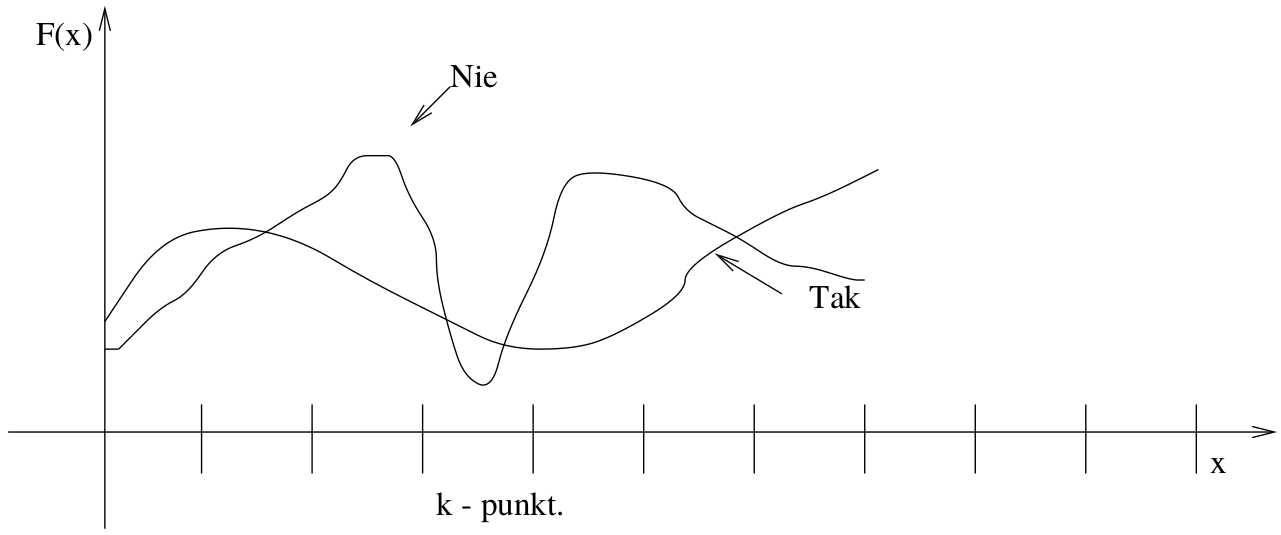
\includegraphics[width=1\textwidth]{img/17/przegladanie_siatki}
  \end{frame}

  \begin{frame}{Przeglądanie siatki \emph{(grid search)}}
    \begin{block}{Realizacja}
      \begin{itemize}
        \item przegląd wartości
        \item wybór najmniejszej $ \to $ odległości od minimum
        $ 0 \leq \frac{\Delta x}{2} $
      \end{itemize}
    \end{block}
    \begin{block}{Wady}
      \begin{itemize}
        \item nie może być stosowana dla $ \infty $ przedziału
        \item nieefektywna $ \to $ nie "uczy się", własności funkcji
      \end{itemize}
    \end{block}
  \end{frame}

  \begin{frame}{Przeglądanie siatki \emph{(grid search)}}
    \begin{tabular}{@{} c l c c c @{}}
      & $ 100 $ & punktów & w & 1 -- D \\
      $ \Rightarrow $ Zawężenie obszaru do 1\% $ \Rightarrow $ & $ 100^{2} $ & & w & 2 -- D \\
      & $ 100^{10} $ & & w & 10 -- D \\
    \end{tabular}
  \end{frame}
